% LTeX: language=de-DE
\section{Tree-Walking Interpreter}

\begin{frame}{Tree-Walking Interpreter}
	\begin{itemize}
        \item \emph{Traversiert} den Syntaxbaum
		\item \emph{Interpretiert} das Programm direkt
	\end{itemize}
\end{frame}

\begin{frame}{Felder des Interpreters}
	\Lirsting[float=H, ranges={10-16}, fancyvrb={fontsize=\footnotesize}]{deps/rush/crates/rush-interpreter-tree/src/interpreter.rs}

	\begin{description}
		\item[scopes] Stack von Scopes; jeder Scope weist einem Variablennamen einen Laufzeitwert zu
		\item[functions] Zuweisung von Funktionsnamen zu einer geteilten Referenz zu dem entsprechenden Knoten im Syntaxbaum
	\end{description}
\end{frame}

\begin{frame}{Weitere Typdefinitionen}
	\begin{minipage}{0.6\textwidth}
		\Lirsting[float=H, ranges={6-13, 22-28}, fancyvrb={fontsize=\small}]{deps/rush/crates/rush-interpreter-tree/src/value.rs}
	\end{minipage}
	\hfill
	\begin{minipage}{0.35\textwidth}
		\begin{itemize}
			\item Aufzählung zum Speichern verschiedener Datentypen
			\item Verschiedene Unterbrechungen des Programmflusses
		\end{itemize}
	\end{minipage}
\end{frame}

\begin{frame}{Traversierung}
	\begin{figure}[H]
		\centering
		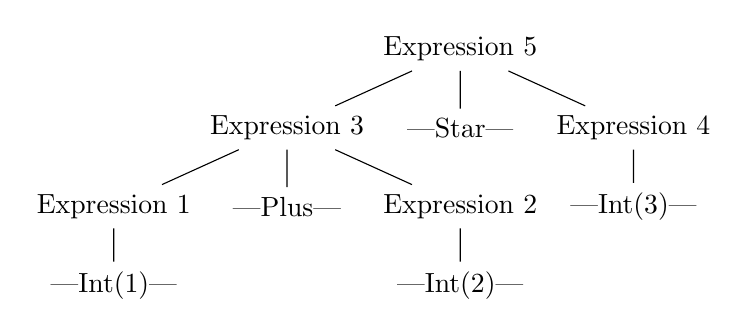
\begin{tikzpicture}[level distance=1cm, sibling distance=2.2cm]
			\node {Expression \encircle{5}}
			child {node {Expression \encircle{3}}
					child {node {Expression \encircle{1}}
							child {node {\Verb|Int(1)|}}}
					child {node {\Verb|Plus|}}
					child {node {Expression \encircle{2}}
							child {node {\Verb|Int(2)|}}}}
			child {node {\Verb|Star|}}
			child {node {Expression \encircle{4}}
					child {node {\Verb|Int(3)|}}};
		\end{tikzpicture}
        \caption{Syntaxbaum zu \enquote{\LirstInline{rush}{1 + 2 * 3}}}
	\end{figure}
\end{frame}

\begin{frame}{Effizienz}
	\begin{minipage}{0.5\textwidth}
		\Lirsting[float=H, fancyvrb={fontsize=\small}]{listings/fib.rush}
	\end{minipage}
	\hfill
	\begin{minipage}{0.45\textwidth}
		\begin{tikzpicture}
			\footnotesize
			\matrix[
			matrix of nodes,
			nodes={minimum height=3ex, draw, text width=4cm},
			row sep=-\pgflinewidth
			](stack){
            \LirstInline{rs}{call_func("fib", vec![3])} \\
			\LirstInline{rs}{visit_block(/* ... */)} \\
			\LirstInline{rs}{visit_expression(/* ... */)} \\
			\LirstInline{rs}{visit_if_expr(/* ... */)} \\
			\LirstInline{rs}{visit_block(/* ... */)} \\
			\LirstInline{rs}{visit_expression(/* ... */)} \\
			\LirstInline{rs}{visit_inifix_expr(/* ... */)} \\
			\LirstInline{rs}{visit_expression(/* ... */)} \\
			\LirstInline{rs}{visit_call_expr(/* ... */)} \\
			\LirstInline{rs}{call_func("fib", vec![2])} \\
			\dots \\
			\LirstInline{rs}{call_func("fib", vec![1])} \\
			};
			\draw[arrow] ([xshift=2.4cm]stack.north) -- ([xshift=2.4cm]stack.south);
		\end{tikzpicture}
	\end{minipage}
\end{frame}
